% =============================================================================
% Architecture figures for the mmCIF post.
%
% Single-file draft. Compile with pdflatex. One figure per page.
% Unified visual language:
%   Hierarchy levels        — monochrome gray gradient
%   Groupings (any kind)    — teal (kind tag distinguishes them)
%   Operators / decoders    — violet
%   State spaces (R1)       — orange
%   Sample axis (R2)        — olive/gold
% =============================================================================

\documentclass[11pt]{article}
\usepackage[a4paper, margin=1.4cm, landscape]{geometry}
\usepackage{forest}
\usepackage{tikz}
\usetikzlibrary{positioning, shapes.geometric, arrows.meta,
                fit, backgrounds, calc, decorations.pathreplacing}
\usepackage{amsmath, amssymb}
\usepackage[hidelinks]{hyperref}

% ---------- Unified palette ----------
\colorlet{H0}{black!16}    % assembly
\colorlet{H1}{black!11}    % entity
\colorlet{H2}{black!7}     % chain
\colorlet{H3}{black!4}     % residue
\colorlet{H4}{black!1}     % atom
\colorlet{rule}{black!50}

\colorlet{accG}{teal!70!black}    % groupings
\colorlet{accO}{violet!70!black}  % operators
\colorlet{accS}{orange!75!black}  % state spaces (R1)
\colorlet{accT}{olive!65!black}   % sample axis (R2)

% ---------- Shared template ----------
\tikzset{
  card/.style    ={draw=rule, rounded corners=2pt, inner sep=4pt,
                   align=center, font=\sffamily\small, line width=0.5pt},
  L0/.style      ={card, fill=H0, minimum width=3.4cm},
  L1/.style      ={card, fill=H1, minimum width=2.6cm},
  L2/.style      ={card, fill=H2, minimum width=2.2cm},
  L3/.style      ={card, fill=H3, minimum width=1.8cm},
  L4/.style      ={card, fill=H4, minimum width=1.4cm,
                   font=\sffamily\footnotesize},
  more/.style    ={draw=rule!60, dashed, rounded corners=2pt, fill=white,
                   font=\sffamily\footnotesize\itshape, text=black!55,
                   minimum width=8mm, inner sep=2pt},
  Lgroup/.style    ={card, fill=white, draw=accG, line width=0.7pt,
                     minimum width=2.6cm},
  Lgroup-cur/.style={Lgroup, dashed},
  Lgroup-cg/.style ={Lgroup, line width=0.9pt},
  Lgroup-het/.style={Lgroup, line width=1.1pt,
                     fill=teal!4},
  Lop/.style     ={card, fill=violet!4, draw=accO, line width=0.7pt,
                   minimum width=2.8cm},
  Lstate/.style  ={card, fill=orange!4, draw=accS, line width=0.6pt,
                   minimum width=1.6cm, font=\sffamily\footnotesize},
  Lvar/.style    ={draw=accS, circle, fill=orange!8, inner sep=1pt,
                   font=\sffamily\footnotesize, minimum size=10mm,
                   align=center, line width=0.6pt},
  Lframe/.style  ={card, fill=olive!4, draw=accT, line width=0.6pt,
                   minimum width=2cm, font=\sffamily\footnotesize},
  contain/.style  ={-, rule, line width=0.5pt},
  member/.style   ={-, accG, line width=0.55pt, dashed},
  bind/.style     ={-Latex, accO, line width=0.7pt},
  nestUnder/.style={-Latex, accS, line width=0.7pt, densely dotted},
  derivedFrom/.style={-Latex, rule, line width=0.55pt, dash dot},
  axisline/.style ={-Latex, accT, line width=0.7pt},
  legcell/.style ={font=\sffamily\footnotesize, anchor=west},
}

\begin{document}
\pagestyle{empty}

% =============================================================================
% Figure 1 — Containment (mmCIF hierarchy)
% =============================================================================
\begin{figure}[p]
\centering
\begin{forest}
  for tree={
    draw=rule, rounded corners=2pt, inner sep=4pt, align=center,
    font=\sffamily\small, line width=0.5pt,
    l sep+=4mm, s sep+=2mm,
    edge={rule, line width=0.5pt},
    grow=south, parent anchor=south, child anchor=north,
  },
  where level=0{fill=H0, minimum width=3.4cm}{},
  where level=1{fill=H1, minimum width=2.6cm}{},
  where level=2{fill=H2, minimum width=2.2cm}{},
  where level=3{fill=H3, minimum width=1.8cm}{},
  where level=4{fill=H4, minimum width=1.4cm,
                font=\sffamily\footnotesize}{},
  moreF/.style={fill=white, draw=rule!60, dashed,
                font=\sffamily\footnotesize\itshape, text=black!55,
                minimum width=8mm, inner sep=2pt},
  [{Assembly}
    [{Entity 1\\ \footnotesize polymer}
      [{Chain A}
        [{Res 1 MET}
          [N] [CA] [C] [\ldots, moreF]
        ]
        [{Res 2 LYS}]
        [\ldots, moreF]
      ]
      [\ldots, moreF]
    ]
    [{Entity 2\\ \footnotesize ligand (ATP)}
      [{Chain L}
        [{ATP}]
      ]
    ]
    [{Entity 3\\ \footnotesize water}
      [{Chain W}
        [{HOH}]
        [\ldots, moreF]
      ]
    ]
    [\ldots, moreF]
  ]
\end{forest}

\vspace{0.6em}
\footnotesize\textbf{Figure 1 — Containment.} The hierarchy layer:
five nested levels with one parent each, exactly as in mmCIF. Dashed
\(\ldots\) cards mark elided multiplicity. Everything else in this
post sits on top of this base.
\end{figure}\clearpage

% =============================================================================
% Figure 2 — Typed groupings (decluttered)
% =============================================================================
\begin{figure}[p]
\centering
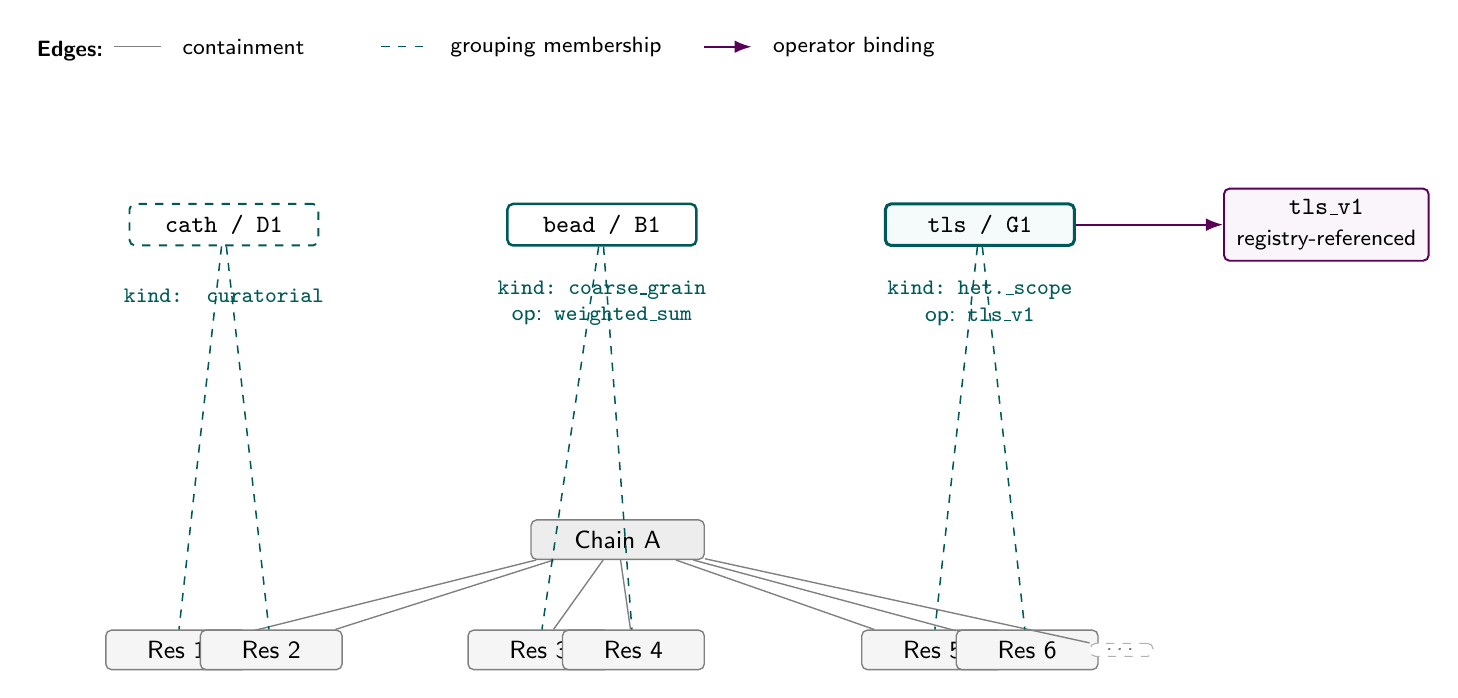
\begin{tikzpicture}

% Legend, isolated at the very top
\begin{scope}[shift={(-7.5, 5.6)}]
  \node[font=\sffamily\footnotesize\bfseries, anchor=west] at (0, 0) {Edges:};
  \draw[contain] (1.1, 0.06) -- (1.7, 0.06);
  \node[legcell] at (1.85, 0.06) {containment};
  \draw[member]  (4.5, 0.06) -- (5.1, 0.06);
  \node[legcell] at (5.25, 0.06) {grouping membership};
  \draw[bind]    (8.6, 0.06) -- (9.2, 0.06);
  \node[legcell] at (9.35, 0.06) {operator binding};
\end{scope}

% Three typed groupings, well separated; coverage non-overlapping for clarity
% (caption notes that real groupings may overlap freely)
\node[Lgroup-cur, align=center, minimum width=2.4cm] (CATH)
  at (-5.0, 3.4) {\texttt{cath / D1}};
\node[font=\sffamily\footnotesize, text=accG, align=center]
  at (-5.0, 2.5) {\texttt{kind: curatorial}};

\node[Lgroup-cg, align=center, minimum width=2.4cm] (CG)
  at (-0.2, 3.4) {\texttt{bead / B1}};
\node[font=\sffamily\footnotesize, text=accG, align=center, text width=3.4cm]
  at (-0.2, 2.4) {\texttt{kind: coarse\_grain}\\
                  \footnotesize op: \texttt{weighted\_sum}};

\node[Lgroup-het, align=center, minimum width=2.4cm] (TLS)
  at (4.6, 3.4) {\texttt{tls / G1}};
\node[font=\sffamily\footnotesize, text=accG, align=center, text width=3.4cm]
  at (4.6, 2.4) {\texttt{kind: het.\_scope}\\
                  \footnotesize op: \texttt{tls\_v1}};

% Operator card on the far right, well separated from the het.scope card
\node[Lop, align=center, minimum width=2.6cm] (OP)
  at (9.0, 3.4) {\texttt{tls\_v1}\\ \footnotesize registry-referenced};
\draw[bind] (TLS.east) -- (OP.west);

% Containment row at the bottom; coverage zones spaced apart
\node[L2] (CA) at (0, -0.6) {Chain A};
\foreach \i/\x in {1/-5.6, 2/-4.4, 3/-1.0, 4/0.2, 5/4.0, 6/5.2} {
  \node[L3] (R\i) at (\x, -2.0) {Res \i};
  \draw[contain] (CA) -- (R\i);
}
\node[more] (Rmore) at (6.4, -2.0) {\ldots};
\draw[contain] (CA) -- (Rmore);

% Membership edges — non-overlapping coverage zones
\draw[member] (CATH) -- (R1);
\draw[member] (CATH) -- (R2);
\draw[member] (CG)   -- (R3);
\draw[member] (CG)   -- (R4);
\draw[member] (TLS)  -- (R5);
\draw[member] (TLS)  -- (R6);

\end{tikzpicture}

\vspace{0.6em}
\footnotesize\textbf{Figure 2 — Typed groupings.}
The Groupings layer is one structural primitive — a sparse bipartite mapping
from hierarchy nodes to a named label set, plus a \texttt{kind} tag — used
three different ways. \texttt{cath / D1} is \texttt{curatorial}: membership
is the contract, the evaluation model never has to touch it. \texttt{bead /
B1} is \texttt{coarse\_grain}: membership plus per-edge weights, with an
operator that lowers it to bead positions. \texttt{tls / G1} is
\texttt{heterogeneity\_descriptor.scope}: membership plus an operator
reference plus a composition tag, lowered when rendering disorder. The
operator (\texttt{tls\_v1}) is registry-referenced — body recoverable from
the spec, shareable across depositions. Coverage zones are drawn
non-overlapping for clarity; in practice a residue can belong to many
groupings simultaneously.
\end{figure}\clearpage

% =============================================================================
% Figure 3 — Regime 1: discrete ensemble
% =============================================================================
\begin{figure}[p]
\centering
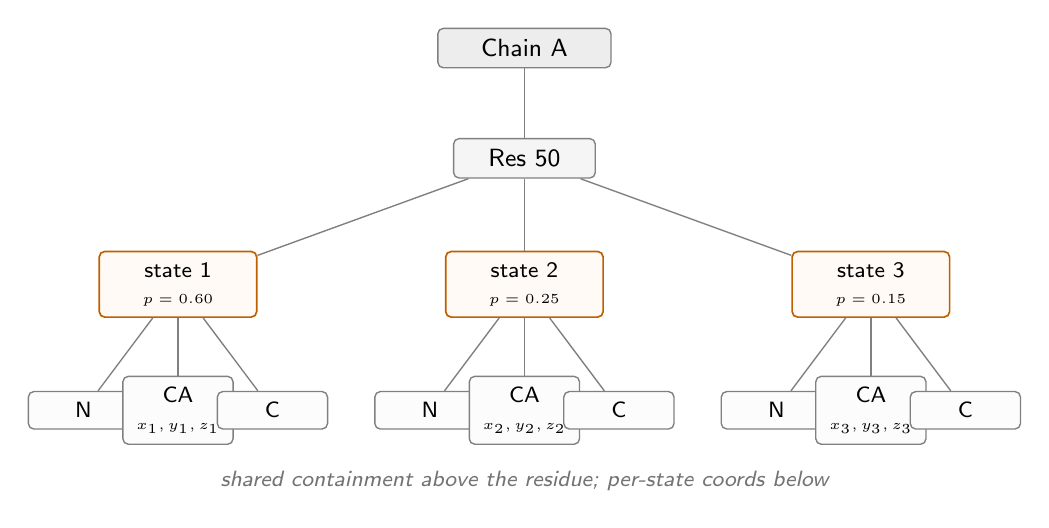
\begin{tikzpicture}

\node[L2] (C) at (0, 2.4) {Chain A};
\node[L3] (R) at (0, 1.0) {Res 50};
\draw[contain] (C) -- (R);

\foreach \s/\x/\pop in {1/-4.4/0.60, 2/0/0.25, 3/4.4/0.15} {
  \node[Lstate, minimum width=2cm] (S\s) at (\x, -0.6)
    {state \s\\ \tiny $p = \pop$};
  \draw[contain] (R) -- (S\s);
  \node[L4] (N\s)  at (\x - 1.2, -2.2) {N};
  \node[L4, align=center] (A\s) at (\x, -2.2)
    {CA\\ \tiny $x_\s,y_\s,z_\s$};
  \node[L4] (Cc\s) at (\x + 1.2, -2.2) {C};
  \draw[contain] (S\s) -- (N\s);
  \draw[contain] (S\s) -- (A\s);
  \draw[contain] (S\s) -- (Cc\s);
}
\node[font=\sffamily\footnotesize\itshape, text=black!55] at (0, -3.1)
  {shared containment above the residue; per-state coords below};

\end{tikzpicture}

\vspace{0.6em}
\footnotesize\textbf{Figure 3 — Regime 1: discrete ensemble.}
A finite, enumerable set of named states, each with its own coords
and a population. NMR bundles, qFit sidechain ensembles, IHM
multi-state models. State count in the tens to low hundreds.
\end{figure}\clearpage

% =============================================================================
% Figure 4 — Regime 2: trajectory
% =============================================================================
\begin{figure}[p]
\centering
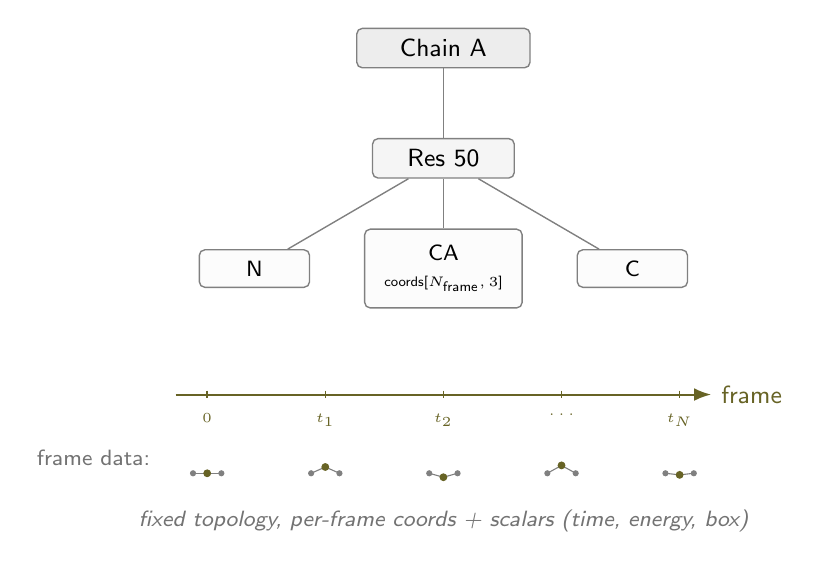
\begin{tikzpicture}

\node[L2] (C) at (0, 2.6) {Chain A};
\node[L3] (R) at (0, 1.2) {Res 50};
\draw[contain] (C) -- (R);

\node[L4] (N)   at (-2.4, -0.2) {N};
\node[L4, align=center, minimum width=2cm, minimum height=1.0cm] (CA)
  at (0, -0.2) {CA\\ \tiny coords[$N_\text{frame}, 3$]};
\node[L4] (Cc)  at ( 2.4, -0.2) {C};
\draw[contain] (R) -- (N);
\draw[contain] (R) -- (CA);
\draw[contain] (R) -- (Cc);

% frame axis
\draw[axisline] (-3.4, -1.8) -- (3.4, -1.8) node[anchor=west, font=\sffamily\small] {frame};
\foreach \t/\lab in {-3/$0$, -1.5/$t_1$, 0/$t_2$, 1.5/$\ldots$, 3/$t_N$} {
  \draw[accT, line width=0.5pt] (\t, -1.75) -- (\t, -1.85);
  \node[font=\sffamily\tiny, text=accT, anchor=north] at (\t, -1.92) {\lab};
}

% per-frame data row
\node[font=\sffamily\footnotesize, text=black!55, anchor=east] at (-3.6, -2.6) {frame data:};
\foreach \t/\jit in {-3/0, -1.5/0.08, 0/-0.05, 1.5/0.10, 3/-0.02} {
  \draw[rule, line width=0.4pt] (\t-0.18, -2.8) -- (\t, -2.8 + \jit) -- (\t+0.18, -2.8);
  \filldraw[rule]  (\t-0.18, -2.8)        circle (0.9pt);
  \filldraw[accT]  (\t,      -2.8 + \jit) circle (1.2pt);
  \filldraw[rule]  (\t+0.18, -2.8)        circle (0.9pt);
}
\node[font=\sffamily\footnotesize\itshape, text=black!55, align=center]
  at (0, -3.4) {fixed topology, per-frame coords + scalars (time, energy, box)};

\end{tikzpicture}

\vspace{0.6em}
\footnotesize\textbf{Figure 4 — Regime 2: trajectory.}
Composition is fixed; the coordinate leaf becomes a dense
\((N_\text{frame}, N_\text{atom}, 3)\) array chunked along the frame
axis, with per-frame scalars riding along. H5MD already specifies the
on-disk shape; the open question is cloud-native chunking.
\end{figure}\clearpage

% =============================================================================
% Figure 5 — Regime 3: continuous landscape
% =============================================================================
\begin{figure}[p]
\centering
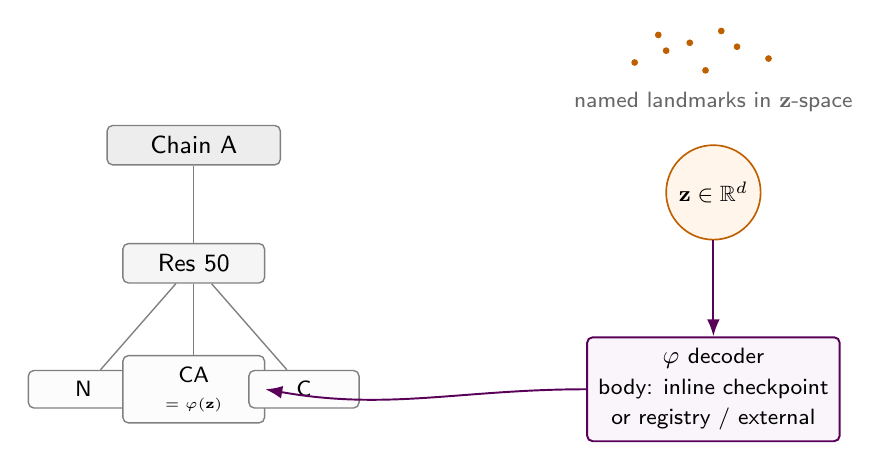
\begin{tikzpicture}

\node[L2] (C) at (-3.6, 2) {Chain A};
\node[L3] (R) at (-3.6, 0.5) {Res 50};
\draw[contain] (C) -- (R);

\node[L4] (N) at (-5.0, -1.1) {N};
\node[L4, align=center, minimum width=1.8cm] (CA)
  at (-3.6, -1.1) {CA\\ \tiny $= \varphi(\mathbf{z})$};
\node[L4] (Cc) at (-2.2, -1.1) {C};
\draw[contain] (R) -- (N);
\draw[contain] (R) -- (CA);
\draw[contain] (R) -- (Cc);

% latent + decoder
\node[Lvar, minimum size=12mm] (Z) at (3, 1.4) {$\mathbf{z}\in\mathbb{R}^d$};
\node[Lop, align=center] (DEC) at (3, -1.1)
  {$\varphi$ \footnotesize decoder\\
   \footnotesize body: inline checkpoint\\
   \footnotesize or registry / external};
\draw[bind] (Z) -- (DEC);
\draw[bind] (DEC.west) to[out=180, in=-10] (CA.east);

% cluster sketch
\node[font=\sffamily\footnotesize, anchor=south, text=black!60] at (3, 2.3)
  {named landmarks in $\mathbf{z}$-space};
\foreach \x/\y in {2.0/3.05, 2.4/3.20, 2.9/2.95, 3.3/3.25,
                   3.7/3.10, 2.7/3.30, 3.1/3.45, 2.3/3.40}
  \filldraw[accS] (\x, \y) circle (1.0pt);

\end{tikzpicture}

\vspace{0.6em}
\footnotesize\textbf{Figure 5 — Regime 3: continuous landscape.}
A collective motion over hundreds of atoms is one low-dimensional
\(\mathbf{z}\) plus a stored decoder \(\varphi\) (cryoDRGN
checkpoint, normal-mode basis, PCA). Named discrete states become
landmarks in \(\mathbf{z}\)-space, not fundamental objects. Mode C
materialization by construction; the decoder body lives inline,
registry, or external.
\end{figure}\clearpage

% =============================================================================
% Figure 6 — Materialization Modes A / B / C
% =============================================================================
\begin{figure}[p]
\centering
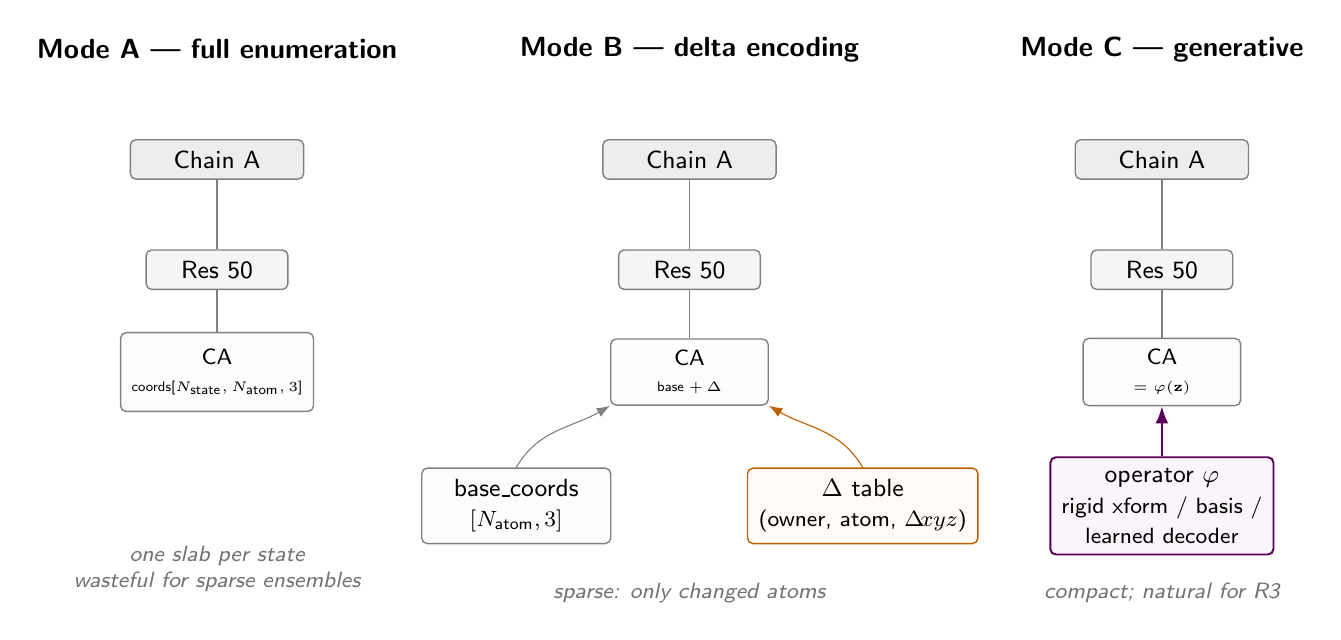
\begin{tikzpicture}

\foreach \mode/\xoff/\label in {A/-6/full enumeration,
                                 B/ 0/delta encoding,
                                 C/ 6/generative} {
  \node[font=\sffamily\bfseries] at (\xoff, 4) {Mode \mode\ — \label};
  \node[L2] (C\mode) at (\xoff, 2.6) {Chain A};
  \node[L3] (R\mode) at (\xoff, 1.2) {Res 50};
  \draw[contain] (C\mode) -- (R\mode);
}

% Mode A
\node[L4, align=center, minimum width=2cm, minimum height=1cm] (CAa)
  at (-6, -0.1)
  {CA\\ \tiny coords[$N_\text{state}, N_\text{atom}, 3$]};
\draw[contain] (RA) -- (CAa);
\node[font=\sffamily\footnotesize\itshape, text=black!55, align=center]
  at (-6, -2.6) {one slab per state\\ wasteful for sparse ensembles};

% Mode B
\node[L4, align=center, minimum width=2cm] (CAb) at (0, -0.1)
  {CA\\ \tiny base $+\,\Delta$};
\draw[contain] (RB) -- (CAb);
\node[card, fill=H4, align=center, minimum width=2.4cm]   (BASE)  at (-2.2, -1.8)
  {base\_coords\\ \footnotesize $[N_\text{atom}, 3]$};
\node[card, fill=orange!4, draw=accS, align=center, minimum width=2.4cm] (DELTA) at (2.2, -1.8)
  {$\Delta$ table\\ \footnotesize (owner, atom, $\Delta\!xyz$)};
\draw[-Latex, rule]  (BASE.north)  to[out=60, in=-150] (CAb.south west);
\draw[-Latex, accS]  (DELTA.north) to[out=120, in=-30] (CAb.south east);
\node[font=\sffamily\footnotesize\itshape, text=black!55, align=center]
  at (0, -2.9) {sparse: only changed atoms};

% Mode C
\node[L4, align=center, minimum width=2cm] (CAc) at (6, -0.1)
  {CA\\ \tiny $= \varphi(\mathbf{z})$};
\draw[contain] (RC) -- (CAc);
\node[Lop, align=center] (OP) at (6, -1.8)
  {operator $\varphi$\\
   \footnotesize rigid xform / basis /\\
   \footnotesize learned decoder};
\draw[bind] (OP.north) -- (CAc.south);
\node[font=\sffamily\footnotesize\itshape, text=black!55, align=center]
  at (6, -2.9) {compact; natural for R3};

\end{tikzpicture}

\vspace{0.6em}
\footnotesize\textbf{Figure 6 — Materialization Modes A / B / C.}
Same containment, three storage strategies for the coordinate leaf.
\textbf{A} stores every state, \textbf{B} stores a base plus sparse
$\Delta$s, \textbf{C} stores an operator applied to a compact input.
Materialization is a per-scope storage choice, independent of the
heterogeneity regime.
\end{figure}\clearpage

% =============================================================================
% Figure 7 — Composition (placeholder for ECHT figure next iteration)
% =============================================================================
\begin{figure}[p]
\centering
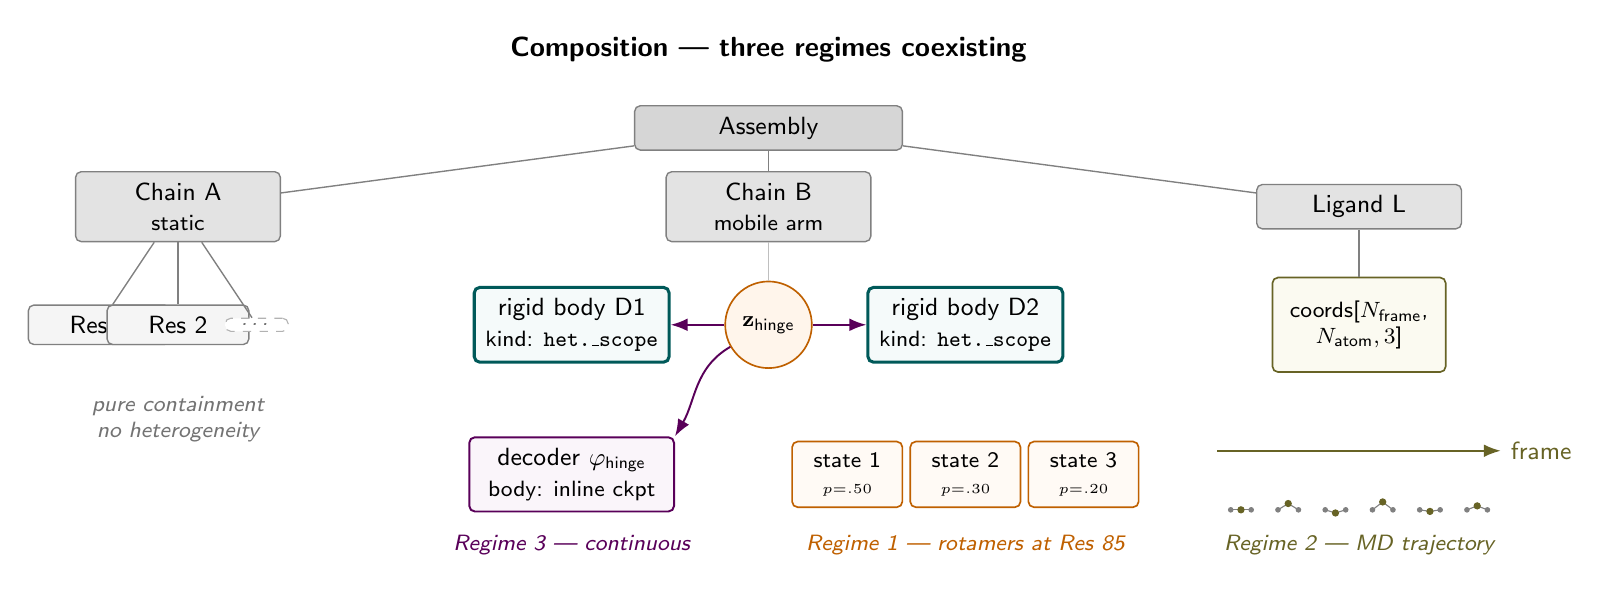
\begin{tikzpicture}

\node[font=\sffamily\bfseries] at (0, 5)
  {Composition — three regimes coexisting};

% assembly + 3 entity columns
\node[L0] (AS) at (0, 4) {Assembly};
\node[L1] (EA) at (-7.5, 3) {Chain A\\ \footnotesize static};
\node[L1] (EB) at ( 0,   3) {Chain B\\ \footnotesize mobile arm};
\node[L1] (EL) at ( 7.5, 3) {Ligand L};
\draw[contain] (AS) -- (EA);
\draw[contain] (AS) -- (EB);
\draw[contain] (AS) -- (EL);

% Chain A — pure containment
\node[L3] (RA1) at (-8.5, 1.5) {Res 1};
\node[L3] (RA2) at (-7.5, 1.5) {Res 2};
\node[more] (RAx) at (-6.5, 1.5) {\ldots};
\draw[contain] (EA) -- (RA1);
\draw[contain] (EA) -- (RA2);
\draw[contain] (EA) -- (RAx);
\node[font=\sffamily\footnotesize\itshape, text=black!55, align=center]
  at (-7.5, 0.3) {pure containment\\ no heterogeneity};

% Chain B — Regime 3 (hinge over rigid bodies) + Regime 1 (rotamer at Res 85)
\node[Lgroup-het, align=center, minimum width=2cm] (D1) at (-2.5, 1.5)
  {rigid body D1\\ \footnotesize kind: \texttt{het.\_scope}};
\node[Lvar, minimum size=11mm] (zH) at ( 0, 1.5) {$\mathbf{z}_\text{hinge}$};
\node[Lgroup-het, align=center, minimum width=2cm] (D2) at ( 2.5, 1.5)
  {rigid body D2\\ \footnotesize kind: \texttt{het.\_scope}};
\draw[bind] (zH) -- (D1);
\draw[bind] (zH) -- (D2);
\draw[contain, black!25] (EB) -- (zH);

\node[Lop, align=center, minimum width=2.6cm] (DEC) at (-2.5, -0.4)
  {decoder $\varphi_\text{hinge}$\\
   \footnotesize body: inline ckpt};
\draw[bind] (zH) to[out=-150, in=60] (DEC.north east);
\node[font=\sffamily\footnotesize\itshape, text=accO, align=center]
  at (-2.5, -1.3) {Regime 3 — continuous};

\node[Lstate, minimum width=1.4cm] (S1) at (1.0, -0.4) {state 1\\ \tiny $p{=}.50$};
\node[Lstate, minimum width=1.4cm] (S2) at (2.5, -0.4) {state 2\\ \tiny $p{=}.30$};
\node[Lstate, minimum width=1.4cm] (S3) at (4.0, -0.4) {state 3\\ \tiny $p{=}.20$};
\node[font=\sffamily\footnotesize\itshape, text=accS, align=center]
  at (2.5, -1.3) {Regime 1 — rotamers at Res 85};

% Ligand L — Regime 2 trajectory
\node[Lframe, align=center, minimum width=2.2cm, minimum height=1.2cm] (LT)
  at (7.5, 1.5) {coords[$N_\text{frame}$,\\ \footnotesize $N_\text{atom}, 3$]};
\draw[contain] (EL) -- (LT);
\draw[axisline] (5.7, -0.1) -- (9.3, -0.1) node[anchor=west, font=\sffamily\small] {frame};
\foreach \t/\jit in {6.0/0, 6.6/0.08, 7.2/-0.04, 7.8/0.10, 8.4/-0.02, 9.0/0.05} {
  \draw[rule, line width=0.4pt] (\t-0.13, -0.85) -- (\t, -0.85 + \jit) -- (\t+0.13, -0.85);
  \filldraw[rule] (\t-0.13, -0.85)        circle (0.8pt);
  \filldraw[accT] (\t,      -0.85 + \jit) circle (1.1pt);
  \filldraw[rule] (\t+0.13, -0.85)        circle (0.8pt);
}
\node[font=\sffamily\footnotesize\itshape, text=accT, align=center]
  at (7.5, -1.3) {Regime 2 — MD trajectory};

\end{tikzpicture}

\vspace{0.6em}
\footnotesize\textbf{Figure 7 — Composition: three regimes coexisting.}
A two-chain complex with a bound ligand. Chain A is plain containment.
Chain B carries a Regime 3 hinge motion over two rigid-body scopes
(decoder \(\varphi_\text{hinge}\) acting on a single latent
\(\mathbf{z}_\text{hinge}\)) and a Regime 1 rotamer ensemble at
residue 85. The ligand is a Regime 2 trajectory. Three regimes,
three attachment points in the system, one consistent vocabulary.
\end{figure}\clearpage

% =============================================================================
% Figure 8 — Hierarchical continuous-additive stack (ECHT on 6vxx)
% =============================================================================
\begin{figure}[p]
\centering
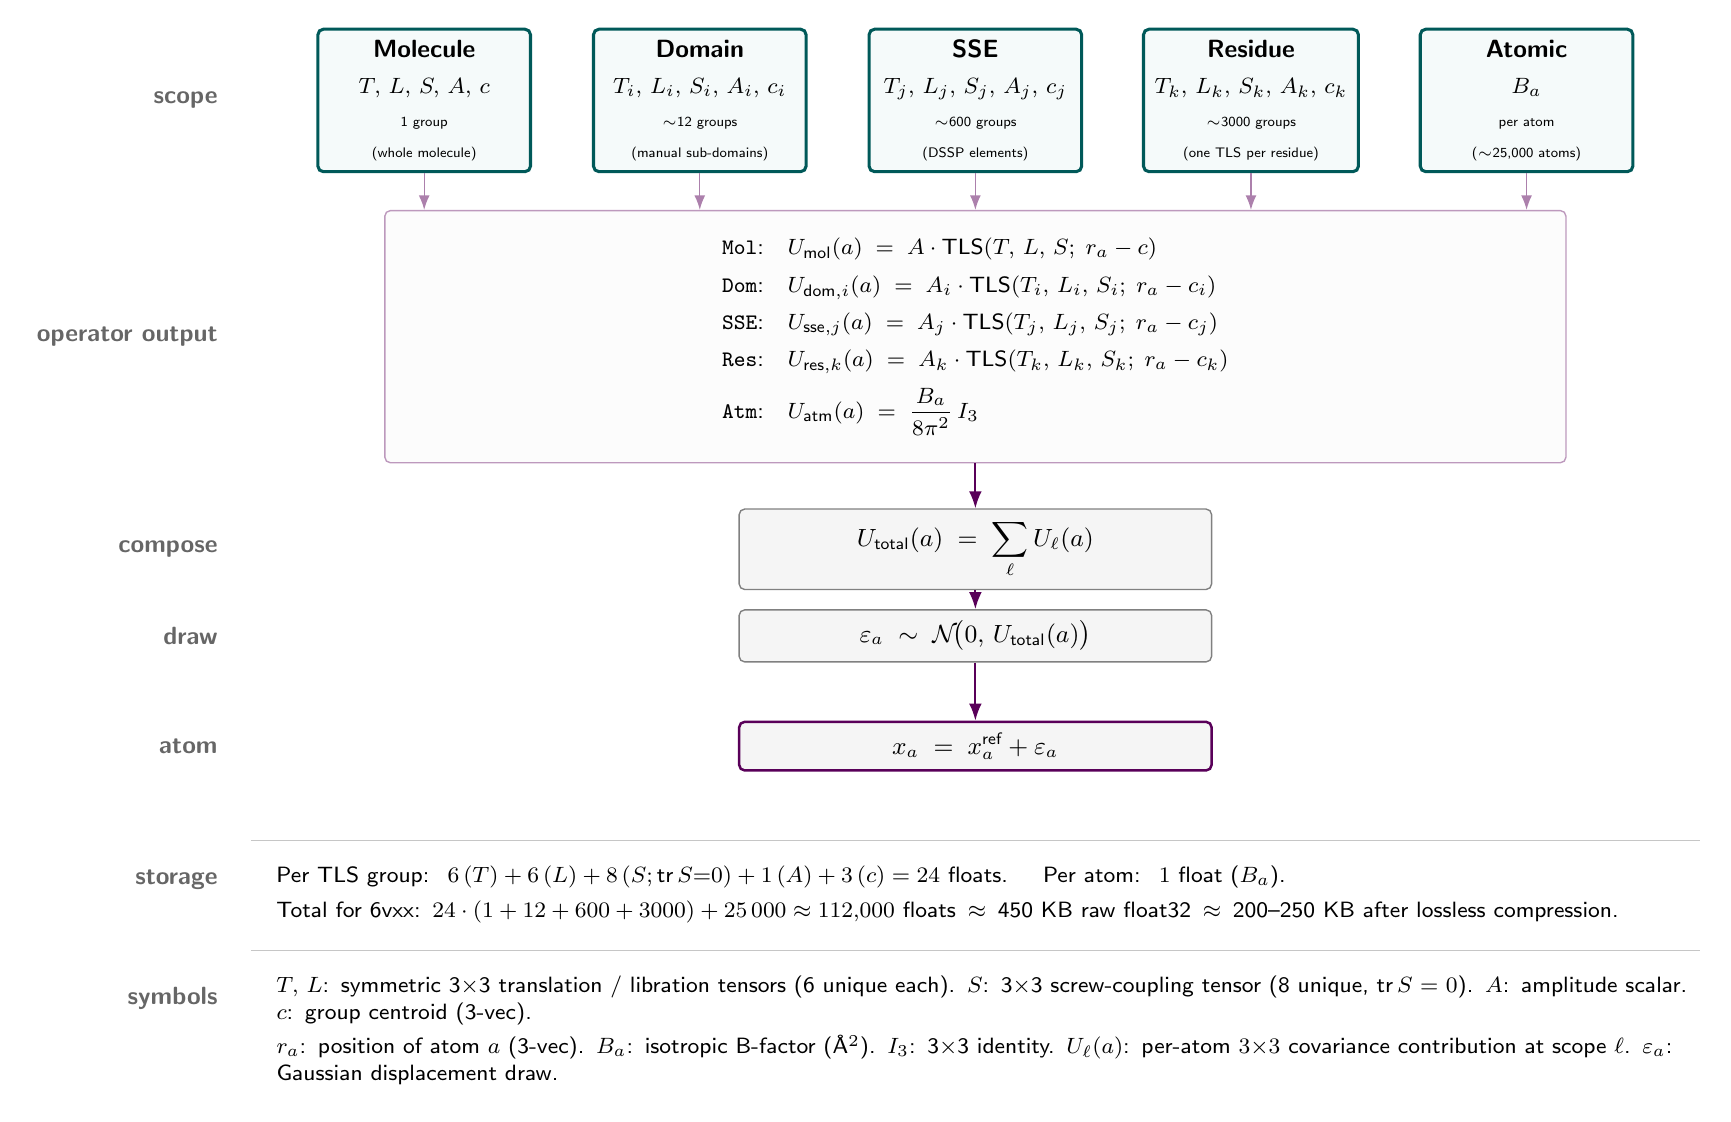
\begin{tikzpicture}

% --- band labels ---
\node[font=\sffamily\small\bfseries, text=black!60, anchor=east] at (-9.5,  6.4) {scope};
\node[font=\sffamily\small\bfseries, text=black!60, anchor=east] at (-9.5,  3.4) {operator output};
\node[font=\sffamily\small\bfseries, text=black!60, anchor=east] at (-9.5,  0.7) {compose};
\node[font=\sffamily\small\bfseries, text=black!60, anchor=east] at (-9.5, -0.4) {draw};
\node[font=\sffamily\small\bfseries, text=black!60, anchor=east] at (-9.5, -1.8) {atom};
\node[font=\sffamily\small\bfseries, text=black!60, anchor=east] at (-9.5, -3.5) {storage};
\node[font=\sffamily\small\bfseries, text=black!60, anchor=east] at (-9.5, -5.0) {symbols};

% --- scope cards: name, variables consumed, group source ---
\node[Lgroup-het, align=center, minimum width=2.7cm, minimum height=1.8cm]
     (mol) at (-7, 6.4)
     {\textbf{Molecule}\\[2pt]
      \footnotesize $T,\, L,\, S,\, A,\, c$\\[1pt]
      \tiny 1 group\\
      \tiny (whole molecule)};

\node[Lgroup-het, align=center, minimum width=2.7cm, minimum height=1.8cm]
     (dom) at (-3.5, 6.4)
     {\textbf{Domain}\\[2pt]
      \footnotesize $T_i,\, L_i,\, S_i,\, A_i,\, c_i$\\[1pt]
      \tiny $\sim$12 groups\\
      \tiny (manual sub-domains)};

\node[Lgroup-het, align=center, minimum width=2.7cm, minimum height=1.8cm]
     (sse) at (0, 6.4)
     {\textbf{SSE}\\[2pt]
      \footnotesize $T_j,\, L_j,\, S_j,\, A_j,\, c_j$\\[1pt]
      \tiny $\sim$600 groups\\
      \tiny (DSSP elements)};

\node[Lgroup-het, align=center, minimum width=2.7cm, minimum height=1.8cm]
     (res) at (3.5, 6.4)
     {\textbf{Residue}\\[2pt]
      \footnotesize $T_k,\, L_k,\, S_k,\, A_k,\, c_k$\\[1pt]
      \tiny $\sim$3000 groups\\
      \tiny (one TLS per residue)};

\node[Lgroup-het, align=center, minimum width=2.7cm, minimum height=1.8cm]
     (atm) at (7, 6.4)
     {\textbf{Atomic}\\[2pt]
      \footnotesize $B_a$\\[1pt]
      \tiny per atom\\
      \tiny ($\sim$25{,}000 atoms)};

% --- operator output: stacked equations ---
\node[card, fill=H4, draw=accO!40, align=left, minimum width=15cm,
      font=\sffamily\footnotesize, inner sep=10pt]
     (ops) at (0, 3.4)
     {\texttt{Mol}:\quad $U_{\text{mol}}(a) \;=\; A \cdot \text{TLS}(T,\, L,\, S;\; r_a - c)$\\[4pt]
      \texttt{Dom}:\quad $U_{\text{dom},i}(a) \;=\; A_i \cdot \text{TLS}(T_i,\, L_i,\, S_i;\; r_a - c_i)$\\[4pt]
      \texttt{SSE}:\quad $U_{\text{sse},j}(a) \;=\; A_j \cdot \text{TLS}(T_j,\, L_j,\, S_j;\; r_a - c_j)$\\[4pt]
      \texttt{Res}:\quad $U_{\text{res},k}(a) \;=\; A_k \cdot \text{TLS}(T_k,\, L_k,\, S_k;\; r_a - c_k)$\\[4pt]
      \texttt{Atm}:\quad $U_{\text{atm}}(a) \;=\; \dfrac{B_a}{8\pi^2}\, I_3$};

% --- arrows: card → operator output block ---
\foreach \src in {mol, dom, sse, res, atm}
  \draw[-Latex, accO!50, line width=0.5pt] (\src.south) -- (\src.south |- ops.north);

% --- compose / draw / atom ---
\node[card, fill=H3, align=center, minimum width=6cm, font=\sffamily\small]
     (sum) at (0, 0.7)
     {$U_{\text{total}}(a) \;=\; \displaystyle\sum_\ell U_\ell(a)$};
\draw[bind] (ops.south) -- (sum.north);

\node[card, fill=H3, align=center, minimum width=6cm, font=\sffamily\small]
     (drawn) at (0, -0.4)
     {$\varepsilon_a \;\sim\; \mathcal{N}\!\bigl(0,\, U_{\text{total}}(a)\bigr)$};
\draw[bind] (sum) -- (drawn);

\node[card, fill=H3, draw=accO, line width=0.9pt, align=center,
      minimum width=6cm, font=\sffamily\small]
     (atom) at (0, -1.8) {$x_a \;=\; x^{\text{ref}}_a + \varepsilon_a$};
\draw[bind] (drawn) -- (atom);

% --- divider before storage ---
\draw[rule!45, line width=0.4pt] (-9.2, -3.0) -- (9.2, -3.0);

% --- storage band ---
\node[font=\sffamily\footnotesize, align=left, text width=18cm, anchor=north west]
     at (-9, -3.2)
     {Per TLS group: $\;6\,(T) + 6\,(L) + 8\,(S; \text{tr}\,S{=}0) + 1\,(A) + 3\,(c) = 24$ floats. \quad
      Per atom: $\;1$ float ($B_a$).\\[3pt]
      Total for 6vxx: $24 \cdot (1 + 12 + 600 + 3000) + 25\,000 \approx 112{,}000$ floats
      $\,\approx\,$ 450 KB raw float32
      $\,\approx\,$ 200--250 KB after lossless compression.};

% --- divider before symbols ---
\draw[rule!45, line width=0.4pt] (-9.2, -4.4) -- (9.2, -4.4);

% --- symbol legend ---
\node[font=\sffamily\footnotesize, align=left, text width=18cm, anchor=north west]
     at (-9, -4.6)
     {$T,\, L$: symmetric 3{$\times$}3 translation / libration tensors (6 unique each).
      $S$: 3{$\times$}3 screw-coupling tensor (8 unique, $\text{tr}\,S = 0$).
      $A$: amplitude scalar.
      $c$: group centroid (3-vec).\\[3pt]
      $r_a$: position of atom $a$ (3-vec).
      $B_a$: isotropic B-factor (\AA$^2$).
      $I_3$: 3{$\times$}3 identity.
      $U_\ell(a)$: per-atom $3{\times}3$ covariance contribution at scope $\ell$.
      $\varepsilon_a$: Gaussian displacement draw.};

\end{tikzpicture}
\vspace{0.6em}

\footnotesize\textbf{Figure 8 — Hierarchical continuous-additive stack
(ECHT applied to PDB 6vxx).} Each scope card shows the parameters its
groups carry plus the source of the group partition: the molecule level is
one TLS for the whole structure; the domain level is one TLS per
manually-defined sub-domain; the secondary-structure level is one TLS per
DSSP-identified helix or strand; the residue level is one TLS per residue
($\sim$3000 in the trimer); and the atomic level keeps a per-atom
isotropic B-factor. Five operator applications turn those parameters into
per-atom $3{\times}3$ covariance contributions. The contributions sum
independently at every atom; one draw from the resulting Gaussian, added
to $x^{\text{ref}}$, gives the concrete atom position.
\end{figure}\clearpage

% =============================================================================
% Figure 9 — Discrete state + continuous disorder (altloc + B-factor)
% =============================================================================
\begin{figure}[p]
\centering
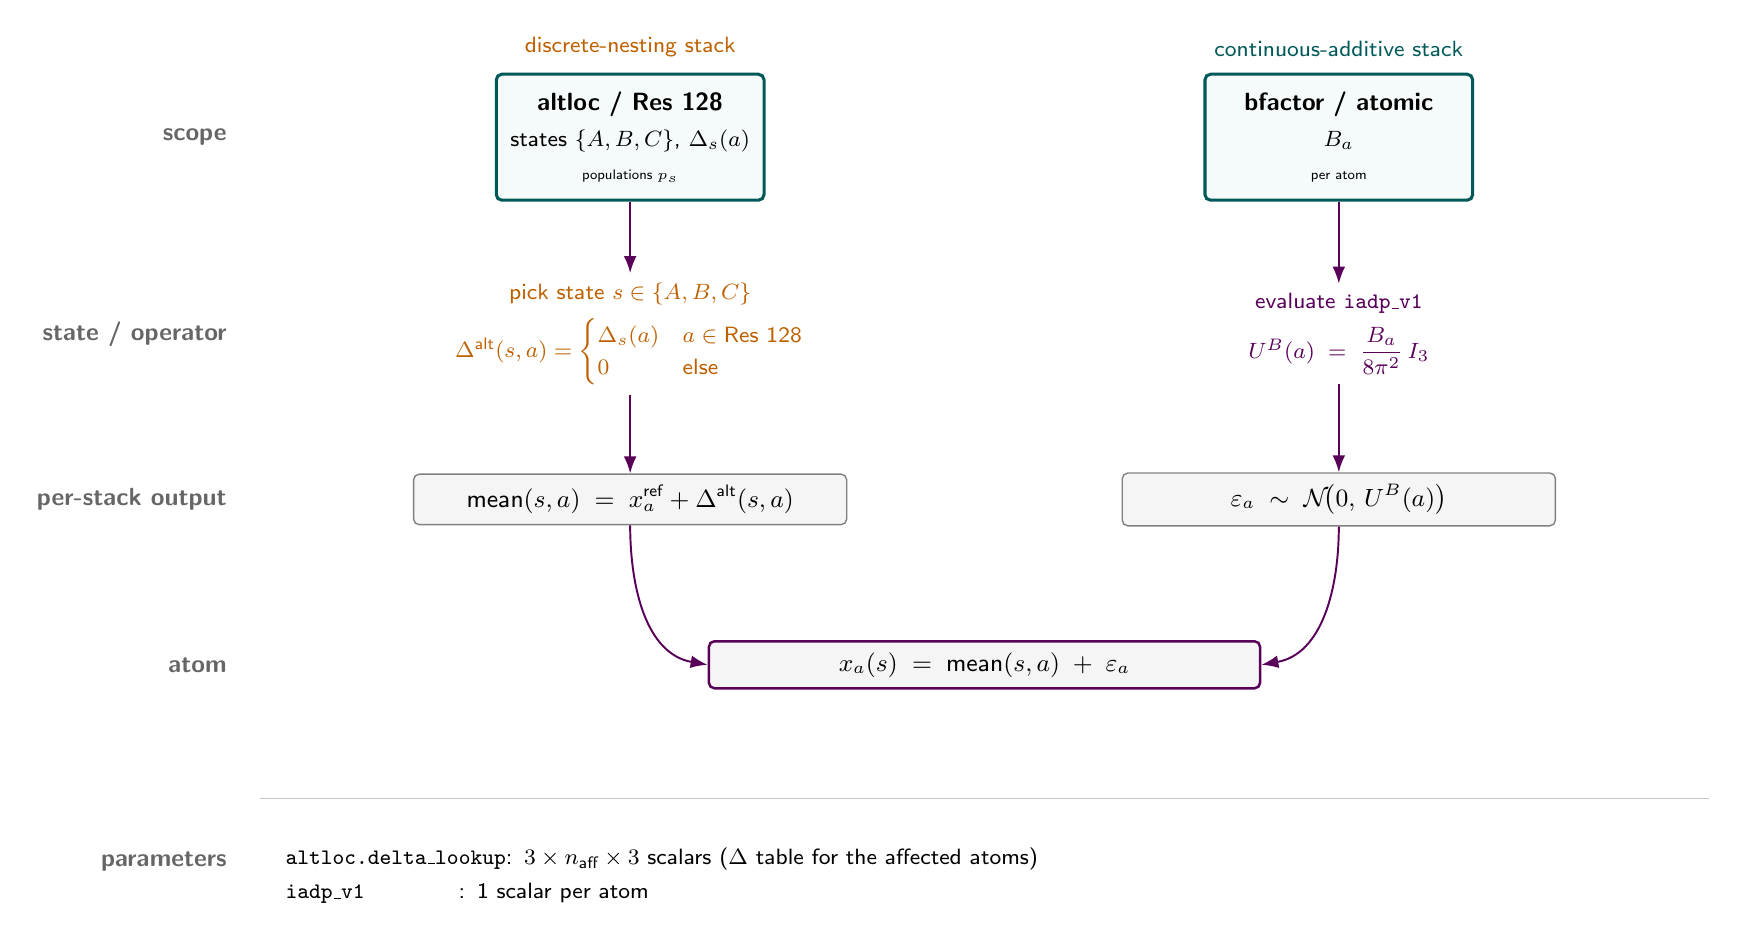
\begin{tikzpicture}

% --- band labels ---
\node[font=\sffamily\small\bfseries, text=black!60, anchor=east] at (-9.5,  6.0) {scope};
\node[font=\sffamily\small\bfseries, text=black!60, anchor=east] at (-9.5,  3.5) {state / operator};
\node[font=\sffamily\small\bfseries, text=black!60, anchor=east] at (-9.5,  1.4) {per-stack output};
\node[font=\sffamily\small\bfseries, text=black!60, anchor=east] at (-9.5, -0.7) {atom};
\node[font=\sffamily\small\bfseries, text=black!60, anchor=east] at (-9.5, -3.2) {parameters};

% --- stack labels ---
\node[font=\sffamily\footnotesize, text=accS, anchor=south]
  at (-4.5, 6.9) {discrete-nesting stack};
\node[font=\sffamily\footnotesize, text=accG, anchor=south]
  at ( 4.5, 6.9) {continuous-additive stack};

% --- concept: two scope groupings ---
\node[Lgroup-het, align=center, minimum width=3.4cm, minimum height=1.6cm]
     (Galt) at (-4.5, 6.0)
     {\textbf{altloc / Res 128}\\[2pt]
      \footnotesize states $\{A, B, C\}$, $\Delta_s(a)$\\[1pt]
      \tiny populations $p_s$};

\node[Lgroup-het, align=center, minimum width=3.4cm, minimum height=1.6cm]
     (Gb)   at ( 4.5, 6.0)
     {\textbf{bfactor / atomic}\\[2pt]
      \footnotesize $B_a$\\[1pt]
      \tiny per atom};

% --- state pick (left) and operator output (right) ---
\node[font=\sffamily\footnotesize, align=center, text=accS] (Salt) at (-4.5, 3.5)
  {pick state $s \in \{A, B, C\}$\\[4pt]
   $\Delta^{\text{alt}}(s, a) =
     \begin{cases}\Delta_s(a) & a\in\text{Res 128}\\ 0 & \text{else}\end{cases}$};

\node[font=\sffamily\footnotesize, align=center, text=accO] (Sb) at (4.5, 3.5)
  {evaluate \texttt{iadp\_v1}\\[4pt]
   $U^B(a) \;=\; \dfrac{B_a}{8\pi^2}\, I_3$};

\draw[bind] (Galt.south) -- (Salt.north);
\draw[bind] (Gb.south)   -- (Sb.north);

% --- per-stack outputs: mean (left) and draw (right) ---
\node[card, fill=H3, align=center, minimum width=5.5cm, font=\sffamily\small]
  (mean) at (-4.5, 1.4)
  {$\text{mean}(s, a) \;=\; x^{\text{ref}}_a + \Delta^{\text{alt}}(s, a)$};

\node[card, fill=H3, align=center, minimum width=5.5cm, font=\sffamily\small]
  (eps) at (4.5, 1.4)
  {$\varepsilon_a \;\sim\; \mathcal{N}\!\bigl(0,\, U^B(a)\bigr)$};

\draw[bind] (Salt) -- (mean);
\draw[bind] (Sb)   -- (eps);

% --- concrete atom: combine mean + eps ---
\node[card, fill=H3, draw=accO, line width=0.9pt, align=center,
      minimum width=7cm, font=\sffamily\small]
  (atom) at (0, -0.7) {$x_a(s) \;=\; \text{mean}(s, a) \;+\; \varepsilon_a$};

\draw[bind] (mean.south) to[out=-90, in=170] (atom.west);
\draw[bind] (eps.south)  to[out=-90, in=10]  (atom.east);

\draw[rule!45, line width=0.4pt] (-9.2, -2.4) -- (9.2, -2.4);

% --- parameters ---
\node[font=\sffamily\footnotesize, align=left, text width=15cm,
      anchor=north west] at (-9, -2.9)
  {\texttt{altloc.delta\_lookup}: $3 \times n_{\text{aff}} \times 3$ scalars
   ($\Delta$ table for the affected atoms)\\[3pt]
   \texttt{iadp\_v1}\hspace{4.0em}: 1 scalar per atom};

\end{tikzpicture}
\vspace{0.6em}

\footnotesize\textbf{Figure 9 — Discrete state plus continuous disorder.}
Two scope groupings sit in different stacks of the evaluation model and
collapse to the same concrete atom. The discrete-nesting stack picks a
state for residue 128, looks up the sparse $\Delta$, and adds it to
$x^{\text{ref}}$ at the affected atoms — atoms outside the residue keep
their reference position. The continuous-additive stack evaluates the
per-atom B-factor through \texttt{iadp\_v1} and draws one Gaussian
displacement per atom. The two streams meet at the final sum: the mean
from the discrete side, the draw from the continuous side, every $a$
independently.
\end{figure}\clearpage

\end{document}
